


\section{Introduction}
\label{sec:introduction}





Large language model (LLM) agents are becoming increasingly capable and autonomous.
Advances in reasoning mechanisms have enabled them to perform multi-step planning, tool use, and problem solving, to the point of surpassing human experts in narrow but cognitively demanding domains such as mathematics competitions (e.g. the International Mathematical Olympiad \citep{LuongLockhart2025}) or programming contests (e.g. the ICPC \citep{LinCheng2025}).
We refer to these as \textit{complex-task/simple-environment} settings: the core challenge lies in solving a difficult reasoning problem, while the environment itself is well-specified, compact, and easily set up.

In contrast, LLM agents continue to struggle with tasks that are individually simple but situated in broad, messy, or dynamic contexts.
Examples include operating vending machines, office workflows, or household tasks \citep{backlund2025vendingbenchbenchmarklongtermcoherence}.
We call these \textit{simple-task/complex-environment} settings.
The reasoning required for each step may be minimal, yet success depends on robustness across a wide distribution of environments, tools, and edge cases.


\begin{figure}
    \vspace{2em}
    \centering
    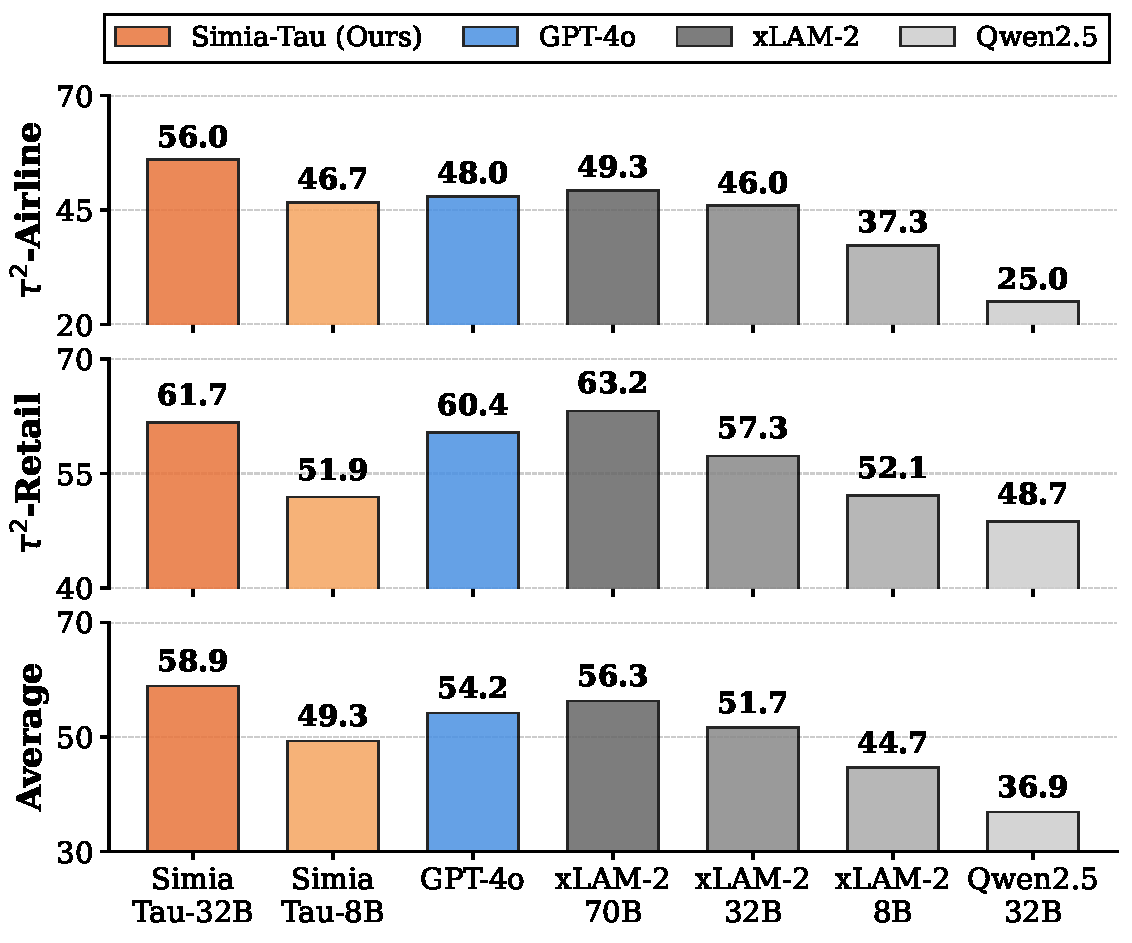
\includegraphics[width=\linewidth]{figs/teaser_new.pdf}
    \caption{Performance of models fine-tuned on our synthetic simulated trajectories without real environment implementations. Our 32B model (based on Qwen2.5-32B-Instruct) surpasses GPT-4o and xLAM-2-70B model and our 8B model (based on Qwen3-8B) outperforms Qwen2.5-32B-Instruct on $\tau^2$-Airline and Retail.}
    \label{fig:teaser}
\end{figure}


We argue that training agents on diverse trajectories spanning a broad range of environments is essential for tackling simple-task/complex-environment challenges \citep{kimiteam2025kimik2openagentic}. Yet building such data at scale is non-trivial. 
Synthetic data generation offers a promising alternative for scalable trajectory creation \citep{patil2023gorillalargelanguagemodel, tang2023toolalpacageneralizedtoollearning, qin2023toolllmfacilitatinglargelanguage, zeng2023agenttuningenablinggeneralizedagent}. However, existing synthesis pipelines are heavily environment-dependent. Traditional approaches construct agent trajectories by implementing environments with explicit tool interfaces and APIs \citep{patil2023gorillalargelanguagemodel, zeng2023agenttuningenablinggeneralizedagent}. While this yields realistic interactions, it tightly couples data generation to environment-specific details, limiting transferability and scalability. Each new environment demands substantial engineering to set up and define tool specifications, making broad coverage impractical.


In this paper, we show that LLMs can act as environment simulators, generating coherent state transitions and tool interactions without access to real environments. This reveals LLMs' capability as environment simulators, exploiting their world modeling abilities to generate coherent environment dynamics, state transitions, and tool interactions without access to the real agent environments.

Building on this observation, we propose: \textbf{Simia-SFT}, a pipeline that synthesizes SFT data by amplifying small seed sets into diverse trajectories in an environment-agnostic manner, and \textbf{Simia-RL}, a framework that enables RL training without real environment implementations by generating LLM simulated feedback. Together, Simia-SFT and Simia-RL enable scalable agent training across diverse tasks without the burden of agentic environment engineering, replacing heavy and brittle environment implementations with flexible LLM-based simulation.



Fine-tuning open models such as \texttt{Qwen3-8B} and \texttt{Qwen2.5-32B-Instruct} on simulated trajectories delivers substantial gains across multiple benchmarks~\citep{wang2024officebench, barres2025tau, liu2023agentbench}. Figure~\ref{fig:teaser} shows that
on $\tau^2$-Bench, our 32B model surpasses GPT-4o and xLAM-2-70B \cite{prabhakar2025apigen} and our 8B model outperforms Qwen2.5-32B-Instruct on Airline and Retail.

In summary, this paper makes the following contributions:
\begin{itemize}[leftmargin=*]
\item \textbf{Simia-SFT Pipeline}. We propose an environment-agnostic trajectory synthesis pipeline that generates complete agent trajectories from small seed sets without executing real environments.
\item \textbf{Simia-SFT Dataset}. The open-source tool-agent training dataset covers multi-turn dialogues and tool use, contributing agentic training and improving agent performance. 
\item \textbf{Simia-RL Framework}. We propose RL on LLM-simulated environments that circumvents agent environment engineering.
\item \textbf{Empirical gains.} Across diverse benchmarks, open models fine-tuned on simulated trajectories and RL on simulated environment yield consistent improvements, surpassing closed-source counterparts on the different benchmarks.
\end{itemize}





These results suggest a practical recipe for agent training: replace environment-specific code with LLM simulators. 
This reframes environment engineering as an amortized prompt-and-schema design question, enabling broader progress in agentic LLM training.
